\documentclass{article}
\usepackage[utf8]{inputenc}
\usepackage[spanish]{babel}
\usepackage{graphicx}
\usepackage{float}
\usepackage{pdfpages}
\graphicspath{{./img/}}

\title{Práctica 3. Primera parte. Ingeniería de requisitos: Análisis y especificación de requisitos}
\author{Eugenio Alcántara García\\
	\and Noelia Escalera Mejías\\
	\and Alejandro Menor Molinero\\
	\and Jesús Torres Sánchez}

\begin{document}
	\maketitle
	
	\section{Modelo conceptual}
	
	\begin{figure}[H]
		\centering
		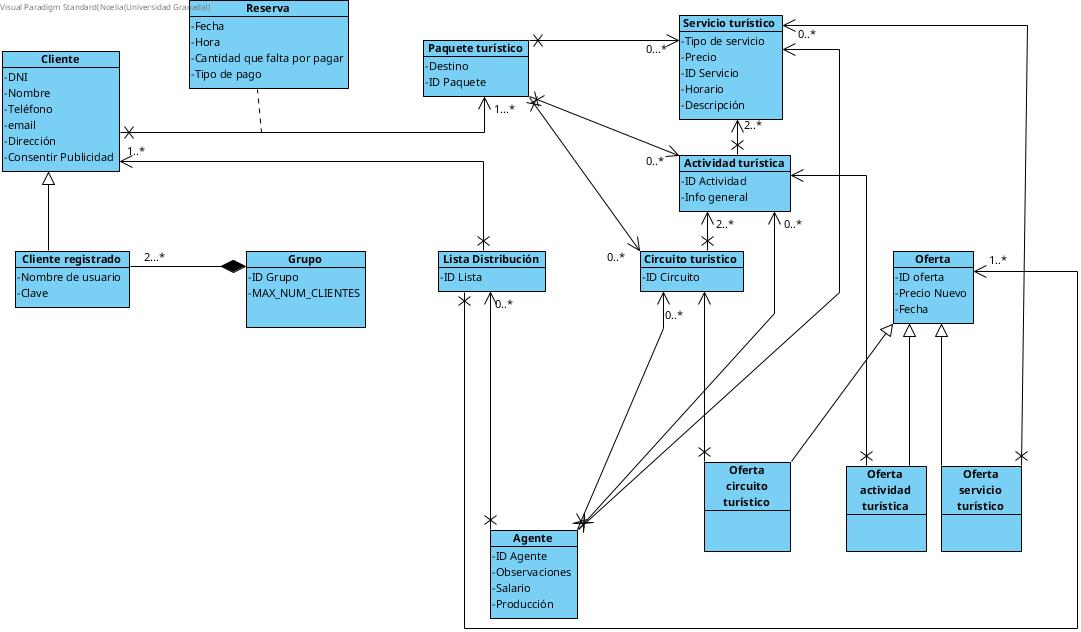
\includegraphics[totalheight=9cm]{Modelo_conceptual}
	\end{figure}
	\newpage
	\section{Diagramas de secuencia}
	\begin{figure}[H]
		\centering
		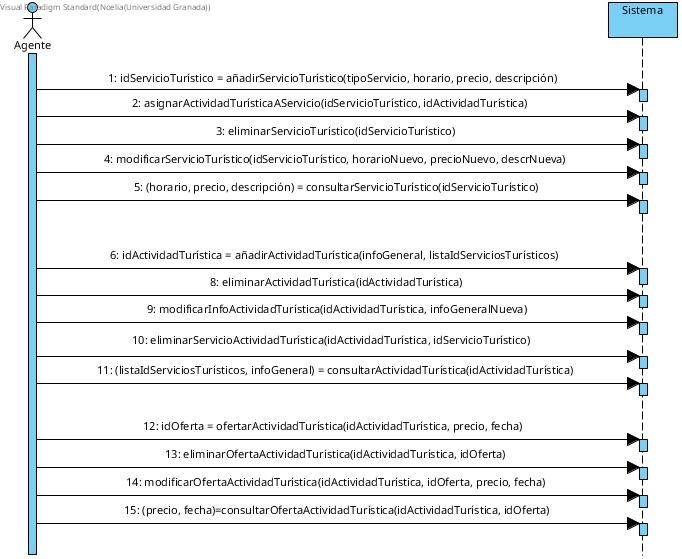
\includegraphics[totalheight=12cm]{Paquete_1}
		\caption{Paquete de Actividades Turísticas}
		\label{fig:p1}
	\end{figure}

	\begin{figure}[H]
		\centering
		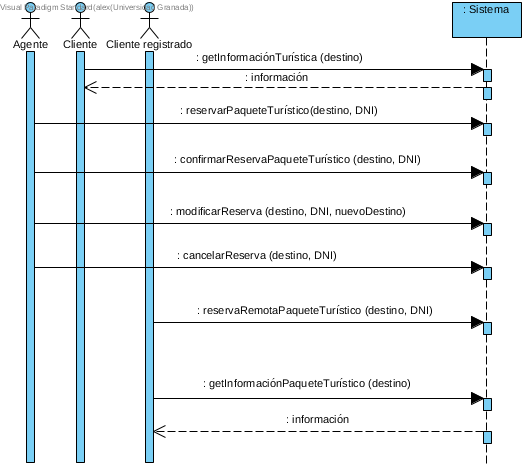
\includegraphics[totalheight=12cm]{Reservas}
		\caption{Paquete de Reservas}
		\label{fig:p2}
	\end{figure}

	\begin{figure}[H]
		\centering
		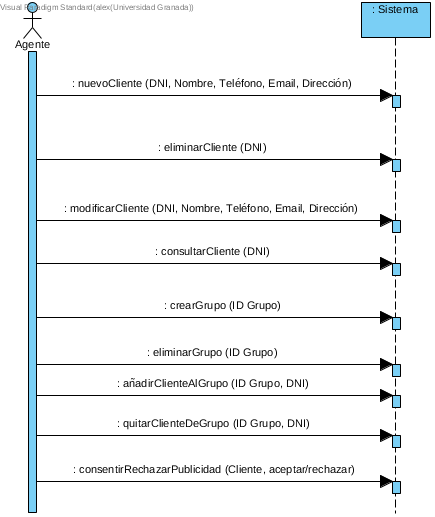
\includegraphics[totalheight=12cm]{Clientes}
		\caption{Paquete de Clientes}
		\label{fig:p3}
	\end{figure}

	\begin{figure}[H]
		\centering
		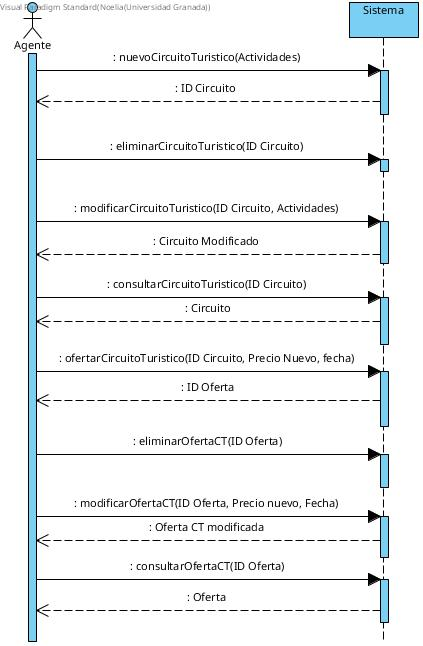
\includegraphics[totalheight=12cm]{Paquete_4}
		\caption{Paquete de Circuitos Turísticos}
		\label{fig:p4}
	\end{figure}

	\begin{figure}[H]
		\centering
		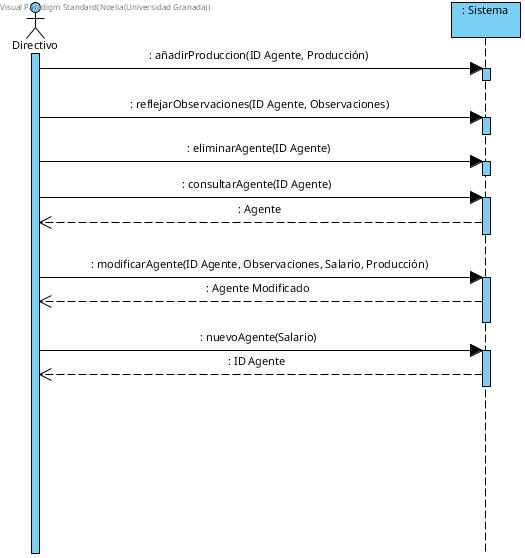
\includegraphics[totalheight=12cm]{Paquete_5}
		\caption{Paquete de Control de Agentes}
		\label{fig:p5}
	\end{figure}

	\begin{figure}[H]
		\centering
		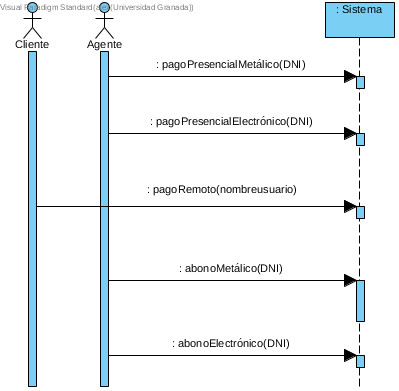
\includegraphics[totalheight=12cm]{Pagos}
		\caption{Paquete de Pagos}
		\label{fig:p6}
	\end{figure}

	\begin{figure}[H]
		\centering
		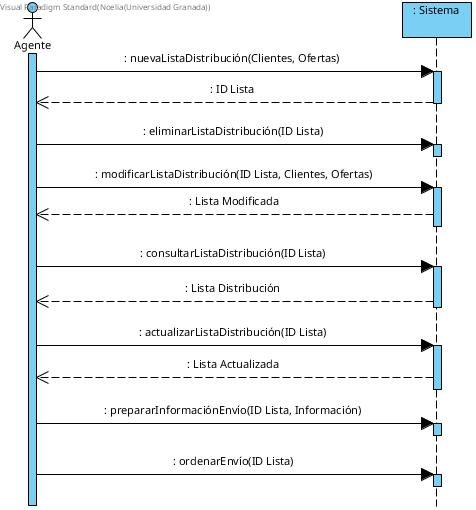
\includegraphics[totalheight=12cm]{Paquete_7}
		\caption{Paquete de Publicidad}
		\label{fig:p7}
	\end{figure}

	\begin{figure}[H]
		\centering
		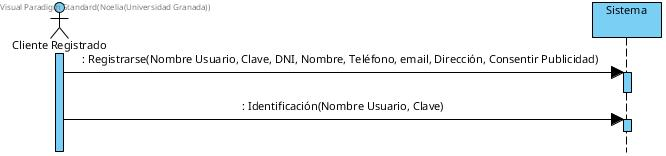
\includegraphics[totalheight=3cm]{Paquete_8}
		\caption{Paquete de Clientes Registrados}
		\label{fig:p8}
	\end{figure}
\end{document}